\chapter{Introduction}\label{introduction}

\section{Introduction}\label{sec:intro}
% topic and context 
Self-Organising Multi-Agent systems provide the perfect framework for the implementation and assessment of theorems surrounding topics such as; psychology, politics and economics. A multi-agent system consists of a number of agents, for whom complexity and objectives can be wide ranging, and the environment that they live in. If allowed to communicate, using some form of agent communication language, these agents can self-organise to achieve a common objective. This can come in many different guises, depending on the environments latitude for deviation from the agent's own principles. 

When the environment is one of a collective survival game, based on an economy of scarcity and collective risks, a multitude of principals can be implemented to equip the agents with the skills to survive, thrive and act according to the not only the self, but also the collective. 

For agents to successfully traverse these game environments, they must embody a number of principles for the management of communities, first introduced by Elinor Ostrom in her 1990 book, Governing The Commons \cite{ostrom2015governing}. Through these, agents can consider such processes as; Institutionalised power, social choice theory, computational justice and alternative dispute resolution. Once again, this hinges upon the agents ability to communicate and aggregate knowledge based on these social interactions. Once complete, informed decisions based upon individual ideals surrounding concepts such as social capital, utility and collective risk can be calculated.

For the purposes of this project, disobedience and divergence from any socially imposed contracts or governmental rules can incur sanctions. However, deceit, lies and manipulations are considered outside of the scope. 
% short introdcution to the module and the objectives/goals of the SOMAS cohort. 
% Some background on Self-Organising Multi-Agent System and its facets
% Ostrom Principals 
% Institutionalised power
% Game theory and strategic interaction 
% Social Choice Theory 
% alternative Dispute Resolution 
% Computational Justice
% Knowledge Agreggation 
% Sanctions and Dissent 

% outline of the report 
This report will present the definition of the game, design considerations that took place and the main objectives. The breakdown of the teams that were created, their members, responsibilities and work flows will be detailed before presenting the implementations required to complete our objectives. Next the game design, DevOps and infrastructure work will be introduced to provide a thorough understanding of the game and its dynamics before agent teams present their strategies, algorithms and implementations. Experimental design results will proceed a discussion on the implications of these results with respect to self-organising multi-agent systems. Finally there will be a conclusion and recommendations for future work. 

\section{Story Line}\label{sec:story line}

% story line
For the implemented game, the following story-line was created: A rag-tag group of rebel peasants find themselves at the bottom of a deep and dark pit. To escape to freedom, the peasants must battle through each rising level of the pit, slaying a number of perilous beasts on their way. With each enemy slayed at the blood soaked hands of the proletarian, they gain access to new and improved weaponry to fight on and never surrender. Once free, the peasants can continue their struggle against the totalitarian dictatorships of the western world, until, in God's good time, the New World, with all its power and might, steps forth to the rescue and the liberation of the old. \cite{churchill} 

To achieve all these goals, peasants must self-organise to survive. This can be done by electing governors, conducting collective risk analysis, assigning common pool resources and performing alternative dispute resolution using institutionalised power. All of these aspects, revolve around the understanding of social choice theory and knowledge aggregation. 


\section{Rules, Attributes \& Artifacts}\label{sec:rules}

The objective of the game is for an Agent to win, individually, by escaping the pit with as many `hit-points' and `health points' as possible, whilst also ensuring that enough of your fellow players survive to start the revolution upon escape. 
For each level within the pit, combat consists of a number of fight rounds which continue until either; the enemy is defeated, or the agents turned into chutney. Within each round, Agents can either; attack, defend, or cower. The first action deals damage to the enemy, the second absorbs damage from the enemy, and the final option skips the round whilst regenerating health and stamina.
Agents will be granted multiple opportunities within fight rounds and pit levels to self-organise. These self-organisational tasks could involve the allocation of loot dropped by a vanquished foe. This particular example occurs at the end of each fight, before advancing to the next level of the pit. Expansion and explanation of each of the tasks will be introduced later in this report. 

Before listing the rules of the games, it is important to give a simple overview of the Agent and enemy attributes as well as the equipment that can be used within the game.  

\subsection{Attributes \& Equipment}

All Agents within the game have the following attributes:

\begin{itemize} 
    \item Health Points ($HP$)
    \item Stamina Points ($ST$)
    \item Attack Base ($A_s$)
    \item Attack Bonus ($A_b$)
    \item Defense Base ($D_s$)
    \item Defense Bonus ($D_b$)
\end{itemize}

Attack and defense bonuses represent the value of the equipment that is currently being used by the agent. The base values are native to all agents and remain constant, the minimum fighting potential of an agent. For the enemy's attributes:

\begin{itemize}
    \item Resilience ($X$)
    \item Damage ($Y$).
\end{itemize}

Equipment is divided into two sections, weapons and potions. Each weapon is of a specific value and can be equipped by an Agent to increase their attack (or defence) potential. There are only two weapon choices:

\begin{itemize}
    \item Sword ($A_b$)
    \item Shield ($D_b$)
\end{itemize}

Swords are used by Agents who attack, and shields are used by Agents who defend. In both cases, their potential would be the combination of both base and bonus attribute values, giving the Total Attack (/Defend). Potions are consumed by Agents to regenerate their attributes, specifically $HP$ and $ST$. Again, there is a specific value assigned to each new potion. 

\begin{itemize}
    \item Health Potion ($P_{hp}$)
    \item Stamina Potion ($P_{st}$)
\end{itemize}

The value mechanisms for all these variables will be outlined in Section \ref{sec: maths}. 

\subsection{Rules}
Now that the basic game variables have been defined, the standard rules of the game can be listed. 

\begin{enumerate}
    \item All agents start with equal $ST$, $HP$
    \item An enemy dies if the aggregate of total attack values is above $X$ at the end of a round - $\sum_{i} (A_bi + A_si) > X_{remaining}$
    \item Enemy damage $Y$ minus the aggregate of $D_s$ is dealt to agents who fight - $\gamma Y - \sum_{i} (D_{bi} + D_{si})$
    \item An agent dies if the damage received is higher than their remaining HP -  $\frac{\gamma Y - \sum_{i} (D_bi + D_si)}{N} > HP$
    \item To attack, an agents stamina must be higher then their total attack - $ST \geq (A_b + A_s)$
    \item To defend, an agents stamina must be higher then their total defence - $ST \geq (D_b + D_s)$
    \item If an agent attacks, their stamina is reduced by their total attack -  $ST = ST - (A_b + A_s)$
    \item If an agent defends, their stamina is reduced by their total defence - $ST = ST - (D_b + D_s)$
    \item If an agent cowers, their stamina and health increases by $HP_c, ST_c$ - $HP = HP + HP_c$, $ST = ST + ST_c$
    \item If all agents cower, all receive damage $\gamma Y$
    \item If, at the end of a round, $N<M$, the game ends 

    \item Agent can hold extra equipment in their inventory
    \item Agents can donate $HP$ to the $HP_{pool}$ at the end of each level
    \item If $HP_{pool} > X$, agents pass level without fighting

    \item Before each round, agents may communicate to decide fight actions and Chairs may issue sanctions to those to defected from the group strategy (if they wish)
    \item At the end of each level, agents may communicate to allocate the common resource pool, elect new governments, trade equipment and resolve any disputes.


\end{enumerate}

% Agent / Enemy Attributes and variables 
% specifications and Rules
% standard rules

Besides these standard rules, there were a number of additions that were made. To add new dimensions to the game's social aspect, agents only have access to granulated views of their fellow agents $HP$ and $ST$ attributes. This addition creates a high degree of uncertainty in agent calculations and inferences which could create interesting outcomes or large changes in group action decisions. An agents inventory will be private, allowing agents to hoard equipment without others knowing. This too allows a higher range of agent strategies and introduces more opportunities for selfishness and exploitation. 

Fight decision strategies are proposed for the whole group and chosen once a majority has been achieved. Deviation from this agreed strategy can result in sanctions, characterised by trade embargos due to a defector being publicly labeled as such. Potential chairs must run for office on a number of policies and are chosen by plurality during governance elections. Finally, an disputes are resolved by the Chairs individual ideals or by the games determination of group utility. All of these decisions attempt to add the concepts of institutionalised power and social choice theory to the game. The specific mechanisms of collective actions and governance will be further detailed in Section \ref{sec: game design}. 

% more nuanced rules and the reasons for these rules 

\section{Aims \& Objectives}\label{sec:aims}

The overarching objective of this project was to test the self-organisational skills of independent agents when placed into a survival, multi-agent environment. We desired to examine the creation and degradation of relationships between agents based on differing ideologies and whether those relationships are based on facets such as; trust, expertise, community contribution or social capital. Another aim was to explore the different types of governments that would be formed by these agents to determine which governance strategy produced the best results, and which caused the most unrest. Further exploration of the range and severity of sanctions placed upon disobedient agents within an unhappy community would complement the evaluation of a Chairs effectiveness to rule. Finally, we attempted to witness the effect of scaling the number of agents within the game on the groups ability to escape the pit and do so as a community. 

For individual agent teams, the objective was to escape the pit whilst achieving the highest utility to the community and the highest utility to the self. When analysing the result of any experimental design, we aim to propose the best agent strategies and the most effective implementation to achieve this strategy, with respect to implementation algorithms. 

An ancillary aim was to assess the effectiveness of our own self-organisation when attempting to achieve these goals. To outline areas of short falling or efficiency and suggest possible improvements that would have led to more efficient work-flows and agents that could defeat more difficult versions of the game. 

As a final objective, we wanted to develop a metric capable of quantifying an agents utility to the group and therefore define a `winner' of the game. 
% enter the aims of the game 
% to test the self-organisational skills of multiple independently designed agents within the game
% to experiemnt with the group of agents and see weather they form relationships based on trust, expertise and community contribution 
% to test the effectiveness of any governments established by the agents, the levels of defections from the group strategy and the severity of any sanctions that are applied. 
% finally to see if scaling the number of agents influences the effectiveness of said governments and the communities progression through the game. 

% finally to attempt to indentify a winner of the game. The definition of the `winner' will be explored in Section.GAMEDESIGN. 


\section{Team Structure}\label{sec:team struct}

To accomplish the goals that have been defined in the previous sub-section, we self-organised into 6 `Agent Teams'. Each team is responsible for implementing their own agent, with their own ideologies and intuitions of how social interactions, coupled with knowledge aggregation, can be utilised to obtain high levels of game proficiency. They will also be in charge of documenting their progress and ultimately writing a report detailing their implementation strategy and experimental design results. Finally, teams must provide code reviews for other teams to maintain consistency of standards and practices. The agent teams, and their members, are defined in Figure \ref{fig:agentteams}. Team leaders impose some hierarchy, and will represent the teams opinions on group decisions as well as updating people on their progress. Overall group decisions will then be decided via consensus of the team leaders. 

\begin{figure}[htb]
    \centering
    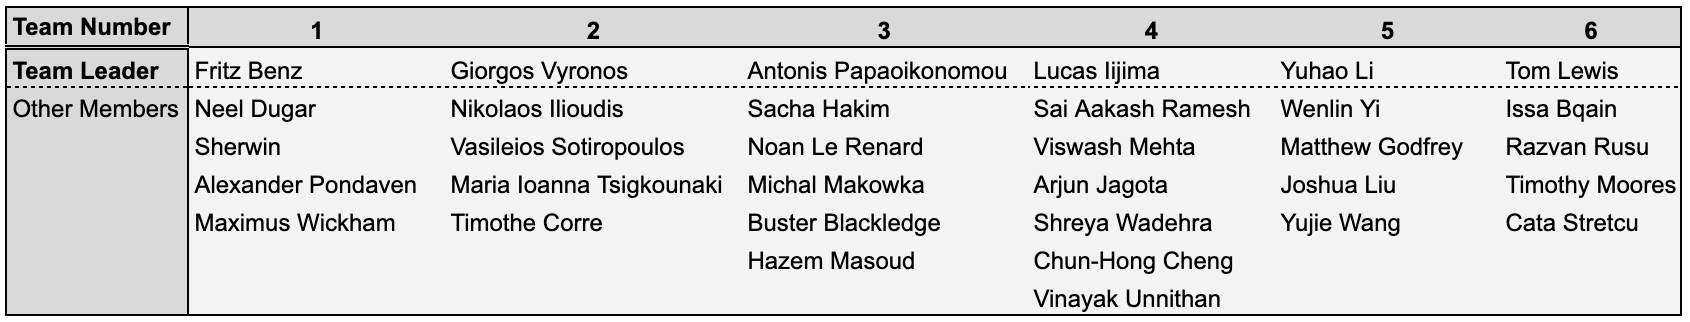
\includegraphics[scale=0.50]{000_introduction/images/subteams.png}
    \caption{Breakdown of the agent teams, their team leaders and members}
    \label{fig:agentteams}
\end{figure}
    
Besides agent teams, there are a number of other sub-teams that are required to complete the project. All of these sub-teams will also be responsible for their output documentation, report section writing and providing regular updates to the group. 
The first is the infrastructure team, and will have the following responsibilities;

\begin{itemize}
    \item Game flow implementation
    \item Agent to server interface
    \item Agent communication standardisation
    \item Front end implementation
\end{itemize}

A major responsibility of this team is the documentation of their functions and methods so that agent teams can easily integrate their agent ideologies within the game. Their work will be explored in detail in Section.INFRA.

The next sub-team is Game Design, who have the following responsibilities;

\begin{itemize}
    \item Game variables algorithmic definitions
    \item Game mechanism definitions 
\end{itemize}

Finally the Development and Operations sub-team was in charge of;

\begin{itemize}
    \item Maintaining version control \& work-flow
    \item Git actions
    \item Unit tests to ensure code integrity
    \item Deployment tools and scripts
\end{itemize}

Each one of these sub-teams were created by agent teams donating 1-2 of their members to each, the breakdown of each team is shown in Figure \ref{fig:subteams}.

\begin{figure}[htb]
    \centering
    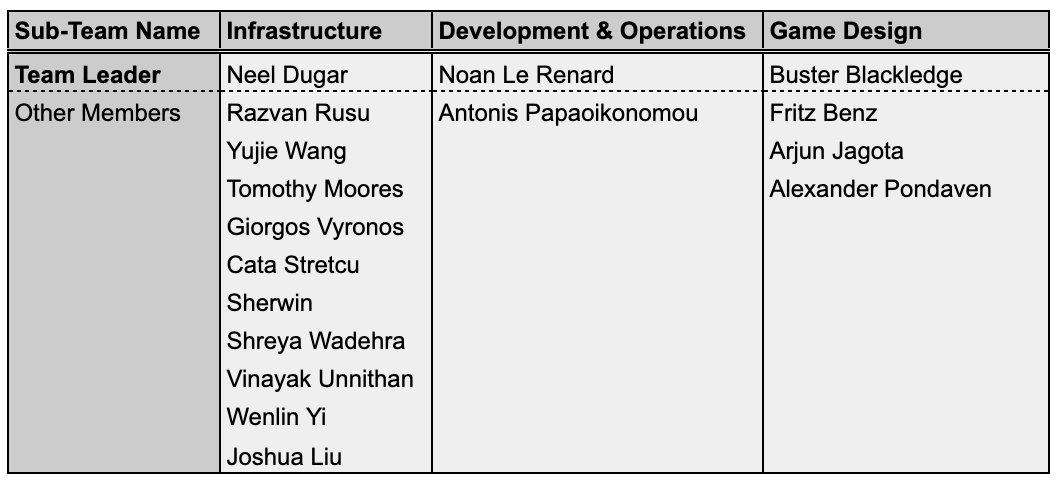
\includegraphics[scale=0.6]{000_introduction/images/agentteams.png}
    \caption{Breakdown of the sub-teams, their team leaders and members}
    \label{fig:subteams}
\end{figure}

%% input the strucutre of each team
% how does the flow of each team work 
%% input each team and who is in each team 

Finally, the overall project was led by Buster Blackledge who was responsible for overall coordination and communication. This structure was used in order to allow everyone to be involved in agent design, whilst allowing all agent teams to have direct access to at least a single member of the infrastructure team. 

As for the decision process. Team leader meetings would discuss design considerations, where each leader represents the opinions of their team members, and make decisions after a consensus had been reached. 